\subsection{Обзор базовой реализации}

В качестве демонстрации полученной модели выбрана реализация визуализации гауссиан с помощью WebGL (браузерный OpenGL) \cite{splat2024}. Так как исходный датасет содержал детальную разметку каждого органа и кости, данный репозиторий был доработан возможностью выделять определенные органы.

WebGL поддерживается многими браузерами, это стало причиной его выбора. Однако у него есть и недостатки --- жесткий графический конвейер, основанный в первую очередь на отображении треугольников, поэтому требуются некоторые хитрости, которые применены оригинальным разработчиком реализации и о которых пойдеть речь дальше.

\begin{figure}[htbp]
	\centering
	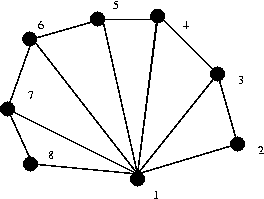
\includegraphics{assets/triangle_fan.png}
	\caption{Визуальная интерпретация работы конвейера в режиме \texttt{TRIANGLE\_FAN} с 8 вершинами}
	\label{fig:triangle-fan}
\end{figure}

Выбран режим отрисовки \texttt{TRIANGLE\_FAN} с 4 вершинами, что эквивалентно рисованию прямоугольника двумя треугольниками (рис. \ref{fig:triangle-fan}). Для отрисовки каждой гауссианы вызывается 4 вершинных шейдера с параметрами
%
\begin{itemize}
	\item позиции: $(-2, -2), (2, -2), (2, 2), (-2, 2)$, соответствующими каждому из углов прямоугольника; при прохождении через вершинный они в неизменном виде передаются во фрагметный, а WebGL их линейно интерполирует; таким образом можно отслеживать в каком месте прямоугольника (внутри которого рисуется гауссиана) находится текущий вызов фрагментного шейдера;
	\item индекс: разделяемый между всеми 4 вершинными шейдерами, он позволяет понять какая гауссиана в данный момент рисуется, важно что буфер в котором хранятся индексы отсортированы в порядке удаления от камеры (до вызова), что позволяет корректно применять формулу альфа блендинга.
\end{itemize}
%
Сами параметры гауссиан хранятся в сжатом виде: для отображения в браузере формат сжат до \texttt{.splat}, который предварительно получается из \texttt{.ply}. Последний хранит гауссианы в том же формате, как они оптимизировались. Например, масштабы как логарифмы, кватернионы не обязательно единичной длины, непрозрачность как логит. Используемый для визуализации формат во первых с целью оптимизации переводит все эти характеристики в буквальные геометрические эквиваленты, а также собирает независимый от взгляда цвет, игнорируя все остальные сферические гармоники.

\begin{table}[htbp]
	\centering
	\begin{tabularx}{\textwidth}{lcX}
		\toprule
		\textbf{Формат} &
		\textbf{Байты} &
		\textbf{Смысл} \\
		\midrule
		\multicolumn{3}{l}{\textit{Пиксель 1}} \\
		
		float32 &
		0-3 &
		Координата центра гауссианы $x$ \\
		
		float32 &
		4-7 &
		Координата центра гауссианы $y$ \\
		
		float32 &
		8-11 &
		Координата центра гауссианы $z$ \\
		
		uint32 &
		12-15 &
		Не используется (заполняется нулём) \\
		
		\midrule
		\multicolumn{3}{l}{\textit{Пиксель 2}} \\
		
		float16 &
		0-1 &
		$4\sigma_{xx}$ \\
		
		float16 &
		2-3 &
		$4\sigma_{xy}$ \\
		
		float16 &
		4-5 &
		$4\sigma_{xz}$ \\
		
		float16 &
		6-7 &
		$4\sigma_{yy}$ \\
		
		float16 &
		8-9 &
		$4\sigma_{yz}$ \\
		
		float16 &
		10-11 &
		$4\sigma_{zz}$ \\
		
		uint8 &
		12 &
		Цвет, канал $R$ \\
		
		uint8 &
		13 &
		Цвет, канал $G$ \\
		
		uint8 &
		14 &
		Цвет, канал $B$ \\
		
		uint8 &
		15 &
		Непрозрачность $\alpha$ \\
		
		\bottomrule
	\end{tabularx}
	\caption{Структура текстуры \texttt{u\_texture}, содержащей параметры гауссиан. Колонка формат говорит как интерпретировать байты.}
	\label{tab:gaussian_texture}
\end{table}

Сами параметры хранятся в текстуре с пикселями RGBA, где каждому каналу выделен uint32, то есть в сумме 16 байт. Два пикселя (32 байта) содержат в себе все параметры гауссианы (таблица \ref{tab:gaussian_texture}).

Задачей вершинного шейдера является извлечь все эти параметры, из них понять в каком прямоугольнике заключена гауссиана (её обрезанная примерно по $\sqrt2 \sigma$ версия), вычислить её цвет $C_\text{vertex}$. Затем фрагметный шейдер по интерполизованным позициям $(p_x, p_y)$ поймет в каком месте прямоугольника находится и выведет итоговый цвет $C = C_\text{vertex} \cdot e^{-(p_x^2 + p_y^2)}$. Чтобы получилась реально спроецированная гауссиана, там, где $\|p\|>2$ цвет не выводится.